%\documentclass[hyperref={pdfpagelabels=false},slidetop,9pt]{beamer}
\documentclass[slidetop,8pt]{beamer}
\usepackage[T1]{fontenc}
\usepackage[utf8]{inputenc}
\newcommand{\id}{71}
\newcommand{\nom}{Théorie des mécanismes}
\newcommand{\sequence}{04}
\newcommand{\nomsequence}{Liaisons entre les solides}
\newcommand{\num}{02}
\newcommand{\type}{KH}
\newcommand{\descrip}{Liaisons équivalentes, hyperstatisme, liaisons en série et en parallèle, théorie des graphes}
\newcommand{\competences}{B2-12: Proposer une modélisation des liaisons avec leurs caractéristiques géométriques. \\ &  B2-13: Proposer un modèle cinématique paramétré à partir d'un système réel, d'une maquette numérique ou d'u \\ &  B2-17: Simplifier un modèle de mécanisme. \\ &  B2-18: Modifier un modèle pour le rendre isostatique. \\ &  C1-04: Proposer une démarche permettant d'obtenir une loi entrée-sortie géométrique.  \\ &  C2-05: Caractériser le mouvement d'un repère par rapport à un autre repère. \\ &  C2-06: Déterminer les relations entre les grandeurs géométriques ou cinématiques. }
\newcommand{\nbcomp}{7}
\newcommand{\systemes}{}
\newcommand{\systemesnum}{}
\newcommand{\systemessansaccent}{}
\newcommand{\ilot}{2}
\newcommand{\ilotstr}{02}
\newcommand{\dossierilot}{\detokenize{Ilot_02 }}

\usepackage{etex}
\usepackage{tikz}
\usepackage[european]{circuitikz}
\usepackage{pgf}
\usepackage[all]{xy}
\usepackage{pgfpages}
\usepackage{graphbox}
\usepackage{pdfpages}
%\usepackage[adobe-utopia]{mathdesign}
\usepackage{ifthen}
\usepackage{cancel}
\usepackage{framed}
\usepackage{subfig}
\usepackage{tabularx}
\usepackage{setspace}
\usepackage{soul}
\usepackage{schemabloc}
\usepackage{eqnarray}
\usepackage[dot, phantomtext]{dashundergaps}
\usepackage{media9}
\usepackage{multimedia}
\usepackage{textcomp}
\usefonttheme[onlymath]{serif}

\author{Renaud Costadoat}
\institute{Lycée Dorian}

\usepackage{multido}
\usepackage{multirow}
\usepackage{multicol} % Portions de texte en colonnes
\usepackage{flafter}%floatants après la référence

\usepackage{color}
\usepackage{xcolor}
\usepackage{colortbl}

\usepackage[gen]{eurosym}
\usepackage{tikz}
%\usepackage{pstricks,pst-node,pst-tree,pst-solides3d}
\usepackage{lmodern}
\usepackage[francais]{babel}
\usepackage{pslatex}
\usetheme{renaud}
\usepackage{times}
\usepackage[frenchmath]{newtxsf} % for sans serif symbols
\renewcommand{\familydefault}{\sfdefault}
%\usepackage{amsfonts}
%\usepackage{amsmath}
%\usepackage{mathastext}
\usepackage{verbatim}
\usepackage{moreverb}
%\usetikzlibrary{arrows,shapes}
\usepackage{graphicx}
\usepackage{psfrag}
\usepackage{wrapfig}
\usepackage{etoolbox}

\definecolor{gris25}{gray}{0.75}
\definecolor{bleu}{RGB}{18,33,98}
\definecolor{bleuf}{RGB}{42,94,171}
\definecolor{bleuc}{RGB}{231,239,247}
\definecolor{rougef}{RGB}{185,18,27}
\definecolor{rougec}{RGB}{255,188,204}%255,230,231
\definecolor{vertf}{RGB}{103,126,82}
\definecolor{vertc}{RGB}{220,255,191}

\setlength\parindent{24pt}
\parskip 7.2pt
\parindent 8pt

\newenvironment{rem}[1][\hsize]%
{%
    \def\FrameCommand
   {%
\rotatebox{90}{\textit{\textsf{Remarque}}} 
       {\color{bleuf}\vrule width 3pt}%
       \hspace{0pt}%must no space.
       \fboxsep=\FrameSep\colorbox{bleuc}%
  }%
    \MakeFramed{\hsize#1\advance\hsize-\width\FrameRestore}%
}%
{\endMakeFramed}%


\newenvironment{savoir}[1][\hsize]%
{%
    \def\FrameCommand
    {%
\rotatebox{90}{\textit{\textsf{Savoir}}} 
        {\color{bleuf}\vrule width 3pt}%
        \hspace{0pt}%must no space.
        \fboxsep=\FrameSep\colorbox{bleuc}%
    }%
    \MakeFramed{\hsize#1\advance\hsize-\width\FrameRestore}%
}%
{\endMakeFramed}%

\newenvironment{prob}[1][\hsize]%
{%
    \def\FrameCommand%
    {%
\rotatebox{90}{\textit{\textsf{Problematique}}} 
        {\color{rougef}\vrule width 3pt}%
        \hspace{0pt}%must no space.
        \fboxsep=\FrameSep\colorbox{rougec}%
    }%
    \MakeFramed{\hsize#1\advance\hsize-\width\FrameRestore}%
}%
{\endMakeFramed}%

\newenvironment{obj}[1][\hsize]%
{%
    \def\FrameCommand%
    {%
\rotatebox{90}{\textit{\textsf{Objectif}}} 
        {\color{vertf}\vrule width 3pt}%
        \hspace{0pt}%must no space.
        \fboxsep=\FrameSep\colorbox{vertc}%
    }%
    \MakeFramed{\hsize#1\advance\hsize-\width\FrameRestore}%
}%
{\endMakeFramed}%

\newenvironment{defi}[1][\hsize]%
{%
    \def\FrameCommand%
    {%
\rotatebox{90}{\textit{\textsf{Definition}}} 
        {\color{bleuf}\vrule width 3pt}%
        \hspace{0pt}%must no space.
        \fboxsep=\FrameSep\colorbox{rougec}%
    }%
    \MakeFramed{\hsize#1\advance\hsize-\width\FrameRestore}%
}%
{\endMakeFramed}%


\newenvironment{hypo}[1][\hsize]%
{%
    \def\FrameCommand%
    {%
\rotatebox{90}{\textit{\textsf{Hypothèse\\}}} 
        {\color{bleuf}\vrule width 3pt}%
        \hspace{0pt}%must no space.
        \fboxsep=\FrameSep\colorbox{bleuc}%
    }%
    \MakeFramed{\hsize#1\advance\hsize-\width\FrameRestore}%
}%
{\endMakeFramed}%


\newenvironment{prop}[1][\hsize]%
{%
    \def\FrameCommand%
    {%
\rotatebox{90}{\textit{\textsf{Propriété}}} 
        {\color{bleuf}\vrule width 3pt}%
        \hspace{0pt}%must no space.
        \fboxsep=\FrameSep\colorbox{bleuc}%
    }%
    \MakeFramed{\hsize#1\advance\hsize-\width\FrameRestore}%
}%
{\endMakeFramed}%

\newenvironment{props}[1][\hsize]%
{%
    \def\FrameCommand%
    {%
\rotatebox{90}{\textit{\textsf{Propriétés}}} 
        {\color{bleuf}\vrule width 3pt}%
        \hspace{0pt}%must no space.
        \fboxsep=\FrameSep\colorbox{bleuc}%
    }%
    \MakeFramed{\hsize#1\advance\hsize-\width\FrameRestore}%
}%
{\endMakeFramed}%

\newenvironment{exemple}[1][\hsize]%
{%
    \def\FrameCommand%
    {%
\rotatebox{90}{\textit{\textsf{Exemple}}} 
        {\color{vertf}\vrule width 3pt}%
        \hspace{0pt}%must no space.
        \fboxsep=\FrameSep\colorbox{vertc}%
    }%
    \MakeFramed{\hsize#1\advance\hsize-\width\FrameRestore}%
}%
{\endMakeFramed}%

\newenvironment{resultat}[1][\hsize]%
{%
    \def\FrameCommand%
    {%
\rotatebox{90}{\textit{\textsf{Résultat}}} 
        {\color{rougef}\vrule width 3pt}%
%        {\color{bleuf}\vrule width 3pt}%
        \hspace{0pt}%must no space.
        \fboxsep=\FrameSep\colorbox{rougec}%
    }%
    \MakeFramed{\hsize#1\advance\hsize-\width\FrameRestore}%
}%
{\endMakeFramed}%

\newenvironment{methode}[1][\hsize]%
{%
    \def\FrameCommand%
    {%
\rotatebox{90}{\textit{\textsf{Méthode\\}}} 
        {\color{rougef}\vrule width 3pt}%
        \hspace{0pt}%must no space.
        \fboxsep=\FrameSep\colorbox{rougec}%
    }%
    \MakeFramed{\hsize#1\advance\hsize-\width\FrameRestore}%
}%
{\endMakeFramed}%

\newenvironment{theo}[1][\hsize]%
{%
    \def\FrameCommand%
    {%
\rotatebox{90}{\textit{\textsf{Théorème\\}}} 
        {\color{rougef}\vrule width 3pt}%
        \hspace{0pt}%must no space.
        \fboxsep=\FrameSep\colorbox{rougec}%
    }%
    \MakeFramed{\hsize#1\advance\hsize-\width\FrameRestore}%
}%
{\endMakeFramed}%

\newenvironment{warn}[1][\hsize]%
{%
    \def\FrameCommand%
    {%
\rotatebox{90}{\textit{\textsf{Attention\\}}} 
        {\color{rougef}\vrule width 3pt}%
        \hspace{0pt}%must no space.
        \fboxsep=\FrameSep\colorbox{rougec}%
    }%
    \MakeFramed{\hsize#1\advance\hsize-\width\FrameRestore}%
}%
{\endMakeFramed}%

% \usepackage{pstricks}
%\usepackage{minitoc}
% \setcounter{minitocdepth}{4}

\setcounter{tocdepth}{2}

% \mtcselectlanguage{french} 

%\usepackage{draftcopy}% "Brouillon"
% \usepackage{floatflt}
\usepackage{psfrag}
%\usepackage{listings} % Permet d'insérer du code de programmation
\renewcommand{\baselinestretch}{1.2}

% Changer la num�rotation des figures :
% ------------------------------------
% \makeatletter
% \renewcommand{\thefigure}{\ifnum \c@section>\z@ \thesection.\fi
%  \@arabic\c@figure}
% \@addtoreset{figure}{section}
% \makeatother
 


%%%%%%%%%%%%
% Définition des vecteurs %
%%%%%%%%%%%%
 \newcommand{\vect}[1]{\overrightarrow{#1}}

%%%%%%%%%%%%
% Définition des torseusr %
%%%%%%%%%%%%

 \newcommand{\torseur}[1]{%
\left\{{#1}\right\}
}

\newcommand{\torseurcin}[3]{%
\left\{\mathcal{#1} \left(#2/#3 \right) \right\}
}

\newcommand{\torseurstat}[3]{%
\left\{\mathcal{#1} \left(#2\rightarrow #3 \right) \right\}
}

 \newcommand{\torseurc}[8]{%
%\left\{#1 \right\}=
\left\{
{#1}
\right\}
 = 
\left\{%
\begin{array}{cc}%
{#2} & {#5}\\%
{#3} & {#6}\\%
{#4} & {#7}\\%
\end{array}%
\right\}_{#8}%
}

 \newcommand{\torseurcol}[7]{
\left\{%
\begin{array}{cc}%
{#1} & {#4}\\%
{#2} & {#5}\\%
{#3} & {#6}\\%
\end{array}%
\right\}_{#7}%
}

 \newcommand{\torseurl}[3]{%
%\left\{\mathcal{#1}\right\}_{#2}=%
\left\{%
\begin{array}{l}%
{#1} \\%
{#2} %
\end{array}%
\right\}_{#3}%
}

 \newcommand{\vectv}[3]{%
\vect{V\left( {#1} \in {#2}/{#3}\right)}
}


\newcommand{\vectf}[2]{%
\vect{R\left( {#1} \rightarrow {#2}\right)}
}

\newcommand{\vectm}[3]{%
\vect{\mathcal{M}\left( {#1}, {#2} \rightarrow {#3}\right)}
}


 \newcommand{\vectg}[3]{%
\vect{\Gamma \left( {#1} \in {#2}/{#3}\right)}
}

 \newcommand{\vecto}[2]{%
\vect{\Omega\left( {#1}/{#2}\right)}
}

\newcommand{\reponse}[1][4]
{
\multido{}{#1}
{
\begin{center}
\makebox[0.9\linewidth]{\dotfill} \end{center}
}}


% }$$\left\{\mathcal{#1} \right\}_{#2} =%
% \left\{%
% \begin{array}{c}%
%  #3 \\%
%  #4 %
% \end{array}%
% \right\}_{#5}}


%  ------------------------------------------
% | Modification du formatage des sections : | 
%  ------------------------------------------

% Grands titres :
% ---------------

\newcommand{\titre}[1]{%
\begin{center}
      \bigskip
      \rule{\textwidth}{1pt}
      \par\vspace{0.1cm}
      
      \textbf{\large #1}
      \par\rule{\textwidth}{1pt}
    \end{center}
    \bigskip
  }

% Supprime le numéro du chapitre dans la numérotation des sections:
% -----------------------------------------------------------------
\makeatletter
\renewcommand{\thesection}{\@arabic\c@section}
\makeatother


% \titleformat{\chapter}[display]
% {\normalfont\Large\filcenter}
% {}
% {1pc}
% {\titlerule[1pt]
%   \vspace{1pc}%
%   \Huge}[\vspace{1ex}%
% \titlerule]


%%%% Chapitres Comme PY Pechard %%%%%%%%%
% numéro du chapitre
\DeclareFixedFont{\chapnumfont}{OT1}{phv}{b}{n}{80pt}
% pour le mot " Chapitre "
\DeclareFixedFont{\chapchapfont}{OT1}{phv}{m}{it}{40pt}
% pour le titre
\DeclareFixedFont{\chaptitfont}{T1}{phv}{b}{n}{25pt}

\definecolor{gris}{gray}{0.75}
\setbeamertemplate{section in toc}[sections numbered]

\newlength{\RoundedBoxWidth}
\newsavebox{\GrayRoundedBox}
\newenvironment{GrayBox}[1][\dimexpr\textwidth-4.5ex]%
   {\setlength{\RoundedBoxWidth}{\dimexpr#1}
    \begin{lrbox}{\GrayRoundedBox}
       \begin{minipage}{\RoundedBoxWidth}}%
   {   \end{minipage}
    \end{lrbox}
    \begin{center}
    \begin{tikzpicture}%
       \draw node[draw=bleuf,fill=bleuc,rounded corners,%
             inner sep=2ex,text width=\RoundedBoxWidth]%
             {\usebox{\GrayRoundedBox}};
    \end{tikzpicture}
    \end{center}}
    
\ifdef{\prive}{\pgfpagesuselayout{2 on 1}[a4paper,border shrink=0mm]}
\ifdef{\prive}{\setbeamertemplate{navigation symbols}{}}
\setbeamertemplate{itemize item}[ball]
%\setbeamertemplate{blocks}[rounded]%[shadow=true]
\setbeamercolor{block title}{fg=white,bg=grisf}        % titre block normal 
\setbeamercolor{block body}{fg=grisf,bg=grisc!50}      % corps block normal
\setbeamercolor{block body alerted}{fg=white,bg=warning}   % idem pour un block alerte

\title{\nom}
\date{S\sequence \ - \type\num}

\begin{document}
\shorthandoff{:!}
\bibliographystyle{abbrvnat-fr}

\usebackgroundtemplate%
{%
    \centering
\includegraphics[width=\paperwidth]{/home/renaud/Documents/Renaud/GitHub/Sciences-Ingenieur/img/fond2}%
}

{
\setbeamertemplate{navigation symbols}{}
\setbeamertemplate{headline}[pagetitre]
\setbeamertemplate{footline}[pagetitre]
\usebackgroundtemplate{\centering
\includegraphics[width=\paperwidth]{/home/renaud/Documents/Renaud/GitHub/Sciences-Ingenieur/img/fond}}
\frame{\titlepage}
}



\section{Introduction}

{\frame{
\frametitle{Introduction}

\begin{savoir}
Vous êtes capables :
\begin{itemize}
 \item de modéliser une action mécanique,
 \item résoudre un problème de statique en utilisant le P.F.S.
\end{itemize}
\end{savoir}

\begin{prob}
Vous devez êtes capables :
\begin{itemize}
  \item modéliser les actions de contact avec frottements.
\end{itemize}
\end{prob}
}}

{\frame{
\frametitle{Lois de Coulomb}

Les lois de Charles de \textbf{Coulomb} permettent de modéliser une action mécanique locale de contact entre deux solides en tenant compte du frottement entre les matériaux en contact.

\vfill

\begin{center}
 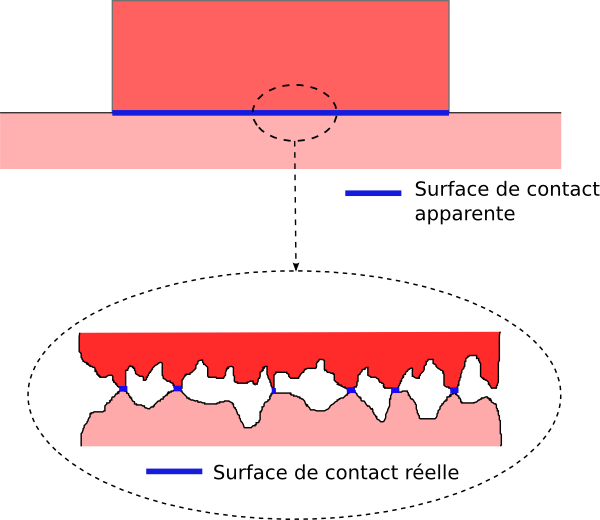
\includegraphics[width=0.5\linewidth]{img/surface_frottement}
\end{center}
}}

{\frame{
\frametitle{Inclinaison de la résultante des efforts de contact}

\begin{itemize}
 \item Le phénomène de frottement apparait lorsque l'on essaye d'induire un glissement relatif entre les deux solides parallèlement au plan de contact,
 \item En considérant la déformation des solides au niveau de leur zone de contact, on constate que la déformation et la répartition des actions élémentaires de contact sont dissymétriques,
 \item Il en résulte que la résultante des actions mécaniques de contact est inclinée par rapport à la normale au plan de contact théorique. 
\end{itemize}

\begin{minipage}{0.5\linewidth}
Remarques : 
\begin{itemize}
 \item La résultante s'incline dans le sens opposé au mouvement relatif des deux solides. Le frottement s'oppose au mouvement relatif 
des solides en contact,
 \item Il n'est pas nécessaire qu'il y ait une vitesse relative pour que la résultante s'incline.
\end{itemize}
\end{minipage}
\hfill
\begin{minipage}{0.4\linewidth}
 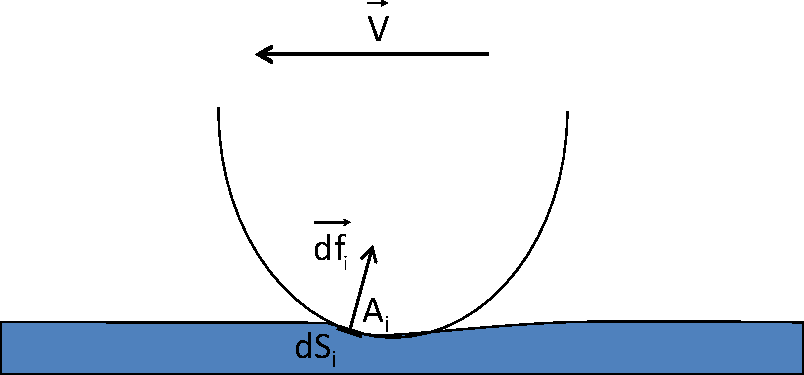
\includegraphics[width=\linewidth]{img/Diapositive10}
\end{minipage}
}}

{\frame{
\frametitle{Modèle de Coulomb}

\textbf{Coefficient de frottement}

\begin{minipage}{0.5\linewidth}
Dans le modèle proposé par Coulomb, on décompose les actions mécaniques de contact en:
\end{minipage}
\hfill
\begin{minipage}{0.4\linewidth}
 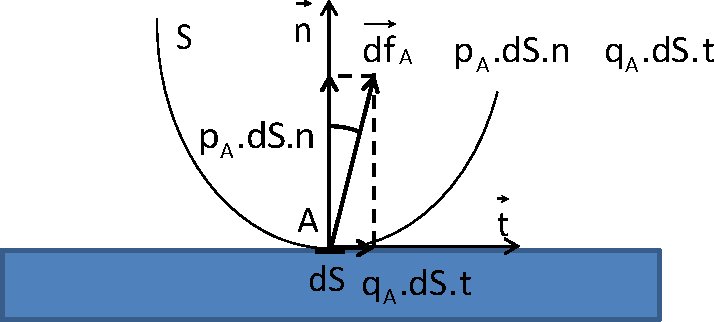
\includegraphics[width=\linewidth]{img/Diapositive11}
\end{minipage}
\begin{itemize}
 \item une composante normale $p.ds.\overrightarrow{n}$ où $p$ est la pression de contact qui règne sur l'élément de surface $ds$ et $\overrightarrow{n}$ la normale à $ds$,
 \item une composante tangentielle $q.ds.\overrightarrow{t}$ où $q$ est la densité tangentielle surfacique d'effort, proportionnelle à $p$,
 \item $p$ et $q$ sont reliés par : $q=f.p$ où $f$ est le coefficient de frottement. 
\end{itemize}
}}

{\frame{
\frametitle{Cône de frottement}

\begin{minipage}{0.5\linewidth}
On défini également l'angle $\varphi$ tel que $tan \varphi=f=\dfrac{q}{p}$. 
Le \textbf{cône de frottement}, dans un contact ponctuel, est alors le cône de demi-angle $\varphi$ dont le sommet est au point de contact et dont l'axe est la normale au contact.
\end{minipage}
\hfill
\begin{minipage}{0.4\linewidth}
 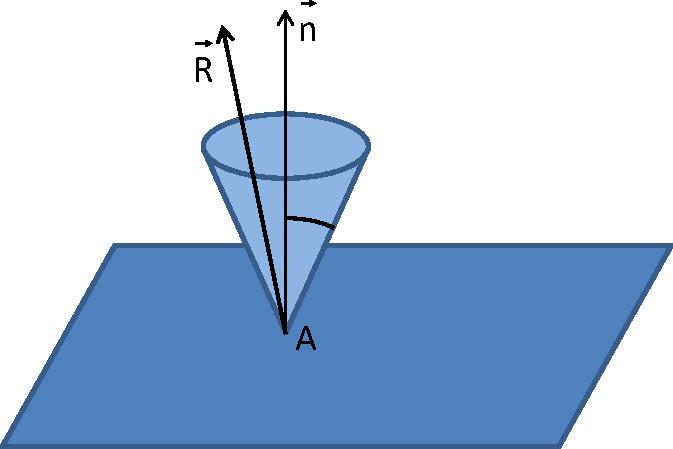
\includegraphics[width=\linewidth]{img/Diapositive12}
\end{minipage}
\begin{itemize}
 \item \textbf{Cas du glissement}: Dans le cas où $\overrightarrow{V_{S/\overline{S}}}\neq \overrightarrow{0}$ (cas du glissement), la résultante des actions mécaniques de contact $\overrightarrow{R_{\overline{S}}\rightarrow S}$ se situe alors sur le cône de frottement et est inclinée dans la direction opposée à $\overrightarrow{V_{S/\overline{S}}}$,
 \item \textbf{Cas du non-glissement (adhérence)}
Dans ce cas $\overrightarrow{V_{S/\overline{S}}}=\overrightarrow{0}$. $\overrightarrow{R_{\overline{S}}\rightarrow S}$ est alors à l'intérieur du cône d'adhérence dont le demi-angle est $\varphi'$, légèrement supérieur à $\varphi$. Sa position exacte dans le cône est déterminée en fonction des conditions d'équilibre du solide.
\end{itemize}
}}

{\frame{
\frametitle{Données numériques}

\begin{tabular}{|c|c|c|}
\hline
Matériaux en contact & Coefficient de frottement f & Coefficient d'adhérence f' \\
\hline
Acier/Acier & 0,1-0,2 & 0,15-0,25 \\
\hline
Acier/Bronze & 0,12-0,2 & 0,15-0,2 \\
\hline
Acier/Ferrodo & 0,2-0,35 & 0,3-0,4 \\
\hline
Acier/PTFE & 0,02-0,08 & 0,1-0,15 \\
\hline
Pneu/Route & 0,3-0,6 & 0,6-1,2 \\
\hline
\end{tabular}

}}


{\frame{
\frametitle{Conclusion}

\begin{savoir}
Vous êtes capables :
\begin{itemize}
  \item modéliser les actions de contact avec frottements.
\end{itemize}
\end{savoir}

\begin{prob}
Vous devez êtes capables :
 \begin{itemize}
  \item d'intégrer l'étude des mouvements à l'étude précédente afin de prendre en compte le Principe Fondamental de la Dynamique,
  \item de prendre en compte la déformation des pièces due à ces efforts.
 \end{itemize} 
\end{prob}
}}

\end{document}